\section{Results and Discussions}

\subsection{Quantum Dots}

\begin{frame}


%Two particle 2D
\begin{figure}
 \begin{center}
 \begin{tabular}{c|lll}
  $\omega$ & $\mathrm{E_{VMC}}$ & $\mathrm{E_{DMC}}$ & $\mathrm{E_{FCI}}$\\
\hline\hline
\multicolumn{4}{c}{} \\
 0.01   & \textbf{0.07}406(5)  & \textbf{0.07383}9(2)  & 0.07383505 \\
 0.1    & \textbf{0.44}130(5)  & \textbf{0.44079}(1)   & 0.44079191 \\
 0.28   & \textbf{1.02}215(5)  & \textbf{1.02164}(1)   & 1.0216441  \\
 0.5    & \textbf{1.6}6021(5)  & \textbf{1.65977}(1)   & 1.6597723  \\
 1.0    & \textbf{3.000}30(5)  & \textbf{3.00000}(1)   & 3.0000001  \\
\cline{1-4}
 \end{tabular}  
 \end{center}
  \caption{Two-particle results for two-dimensional quantum dots compared with FCI results by Veronica K.B. Olsen.}
\end{figure}
\end{frame}


%Two particle 42 56 2D
\begin{frame}

\begin{figure}
 \begin{center}
 \footnotesize
 \begin{tabular}{cc|llll}
 N      &  $\omega$ & $\mathrm{E_{VMC}}$ & $\mathrm{E_{DMC}}$ & $\mathrm{E_{SRG}}$ & $\mathrm{E_{CCSD}}$\\
\hline\hline
\multicolumn{6}{c}{} \\
    42    &   0.1    & 107.881(1)  & 107.6389(2) &- 			& 111.7170 \{8\} \\
          &   0.28   & 220.161(1)  & 219.8426(2) &219.8836 \{14\}	& 222.1401 \{8\} \\
          &   0.5    & 331.002(1)  & 330.6306(2) &330.6485 \{14\}	& 331.8901 \{8\} \\
          &   1.0    & 544.2(8)    & 542.9428(8) &542.9528 \{14\}	& 543.1155 \{18\}\\
\cline{2-6}
\multicolumn{6}{c}{} \\
    56    &   0.1    & 176.269(2) & 175.9553(7)  & -		& 186.1034 \{9\} \\
          &   0.28   & 358.594(2) & 358.145(2)   & -		& 363.2048 \{9\} \\
          &   0.5    & 538.5(6)   & 537.353(2)   & -		& 540.3430 \{9\} \\
          &   1      & 880.2(7)   & 879.3986(6)  & -		& 879.6386 \{17\}\\
\cline{2-6}
 \end{tabular}  
 \end{center}
  \caption{Results for two-dimensional quantum dots 42 and 56 particles compared with SRG results by Sarah Reimann and CCSD results by Christoffer Hirth.}
\end{figure}
\end{frame}

\normalsize

%Two particle 2D
\begin{frame}

\footnotesize
\begin{figure}
 \begin{center}
 \begin{tabular}{cc|rrr}
    N     & $\omega$ & $\mathrm{E_{VMC}}$ & $\mathrm{E_{DMC}}$ & $\mathrm{E_0}$\\
\hline\hline
\multicolumn{5}{c}{} \\
    2     &   0.01   & 0.07939(3)  & 0.079206(3) & -		\\
          &   0.1    & 0.50024(8)  & 0.499997(3) & 0.5        \\
          &   0.28   & 1.20173(5)  & 1.201725(2) & -		\\
          &   0.5    & 2.00005(2)  & 2.000000(2) & 2.0 \\
          &   1.0    & 3.73032(8)  & 3.730123(3) & - \\
\cline{2-5}
\multicolumn{5}{c}{} \\
    8     &   0.1    & 5.7130(6)   & 5.7028(1)   & - 		\\
          &   0.28   & 12.2040(8)  & 12.1927(1)  & -		\\
          &   0.5    & 18.9750(7)  & 18.9611(1)  & -\\
          &   1.0    & 32.6842(8)  & 32.6680(1)  & -\\
\cline{2-5}
\multicolumn{5}{c}{} \\
    20    &   0.1    & 27.316(2)   & 27.2717(2)   & - 		\\
          &   0.28   & 56.440(2)   & 56.3868(2)   & -		\\
          &   0.5    & 85.714(2)   & 85.6555(2)   & - \\
          &   1.0    & 142.951(2)  & 142.8875(2)  & -
 \end{tabular}  
 \end{center}
  \caption{Results for three-dimensional quantum dots compared with exact solutions by M. Taut.}
\end{figure}
\end{frame}

\normalsize


 
 \begin{frame}
  \captionsetup[subfloat]{labelformat=empty}
\begin{figure}
 \begin{center}
  \subfigure[$N=2$]{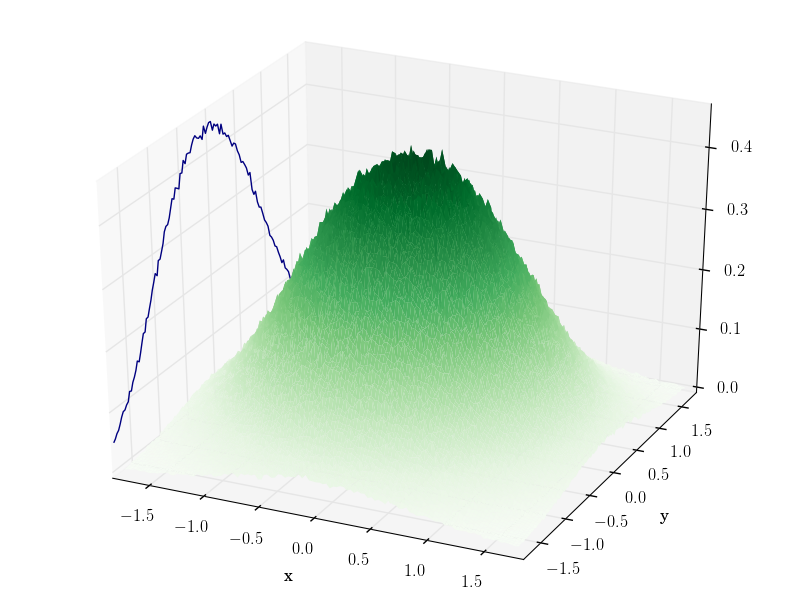
\includegraphics[scale=0.15]{../graphics/OBD/OBD_DMC/dist_out_QDots2c1_3D.png}}
  \subfigure[$N=12$]{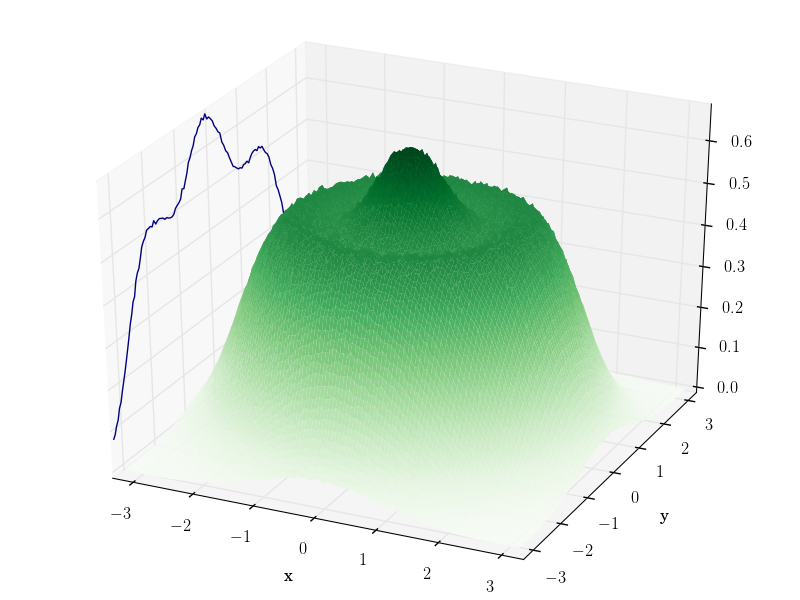
\includegraphics[scale=0.15]{../graphics/OBD/OBD_DMC/dist_out_QDots12c1_3D.png}}
  \subfigure[$N=30$]{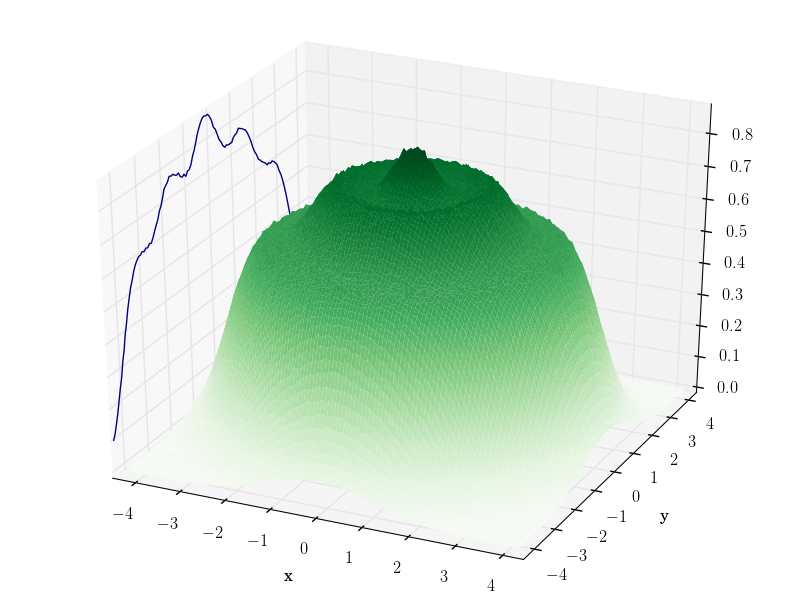
\includegraphics[scale=0.15]{../graphics/OBD/OBD_DMC/dist_out_QDots30c1_3D.png}}\\
  \subfigure[$N=6$]{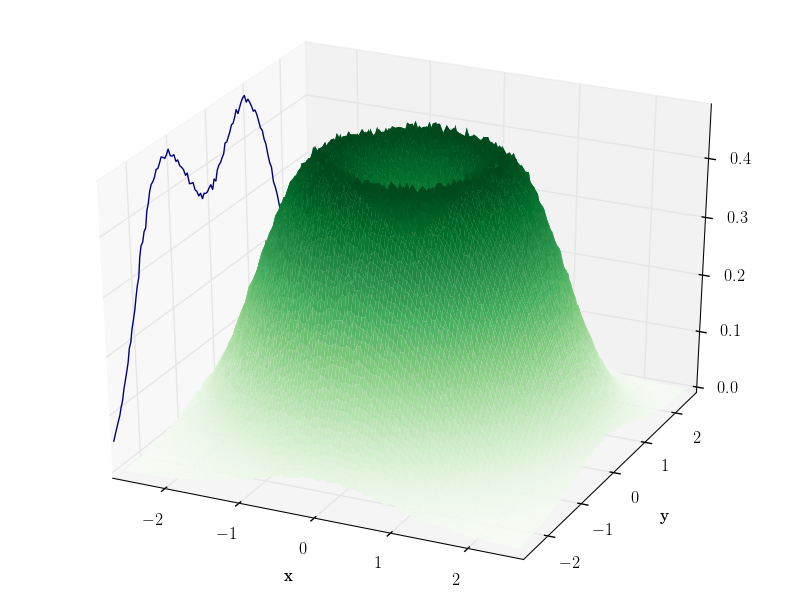
\includegraphics[scale=0.15]{../graphics/OBD/OBD_DMC/dist_out_QDots6c1_3D.png}} 
  \subfigure[$N=20$]{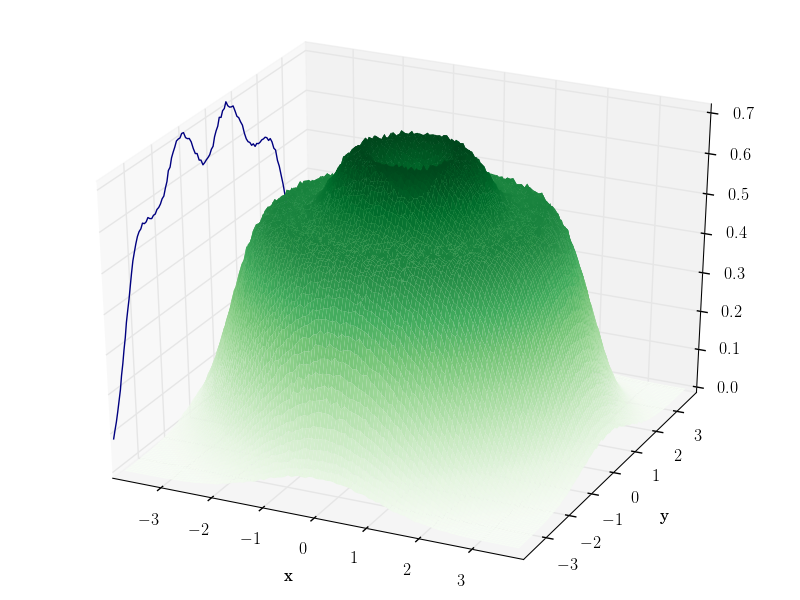
\includegraphics[scale=0.15]{../graphics/OBD/OBD_DMC/dist_out_QDots20c1_3D.png}} 
  \subfigure[$N=42$]{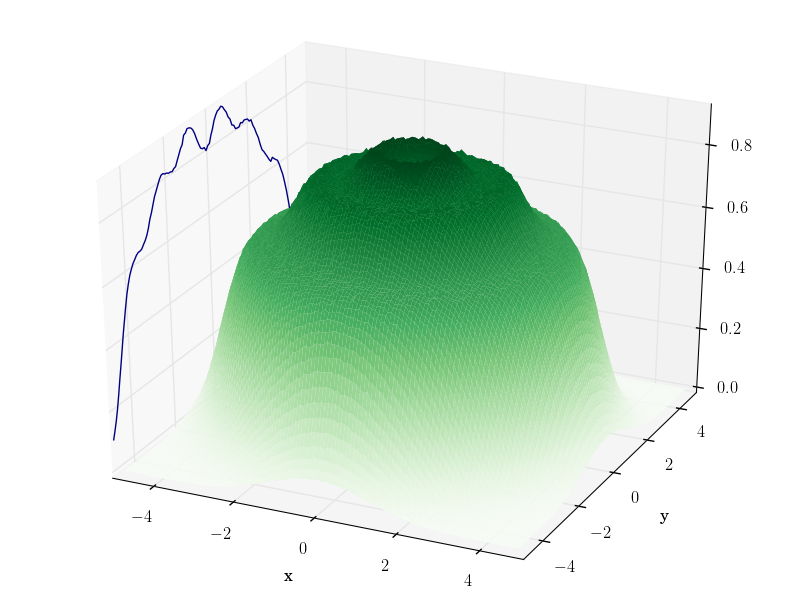
\includegraphics[scale=0.15]{../graphics/OBD/OBD_DMC/dist_out_QDots42c1_3D.png}} \\
  \caption{DMC one-body densities for two-dimensional quantum dots.}
  \label{fig:OBD_DMC_QDOTS_w1} 
 \end{center}
\end{figure}
 \end{frame}

\begin{frame}

\begin{center}
\begin{tabular}{cc}
VMC density & $|\Psi_T(\mathbf{r})|^2$ \\
&  \\
DMC density & $\Phi(\mathbf{r}, \tau)\Psi_T(\mathbf{r})$ \\
&  \\
Pure density & $|\Phi(\mathbf{r}, \tau)|^2$  
\end{tabular}
\end{center}

\end{frame}
 
\begin{frame}

\begin{figure}
 \begin{center}
 \begin{tabular}{cc|c}
   \subfigure{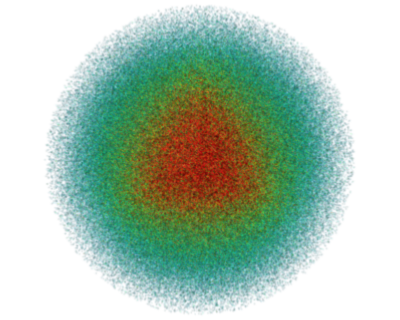
\includegraphics[scale=0.15]{../graphics/OBD/OBD_Q3D/QD2w1_3D.png}} &
   \subfigure{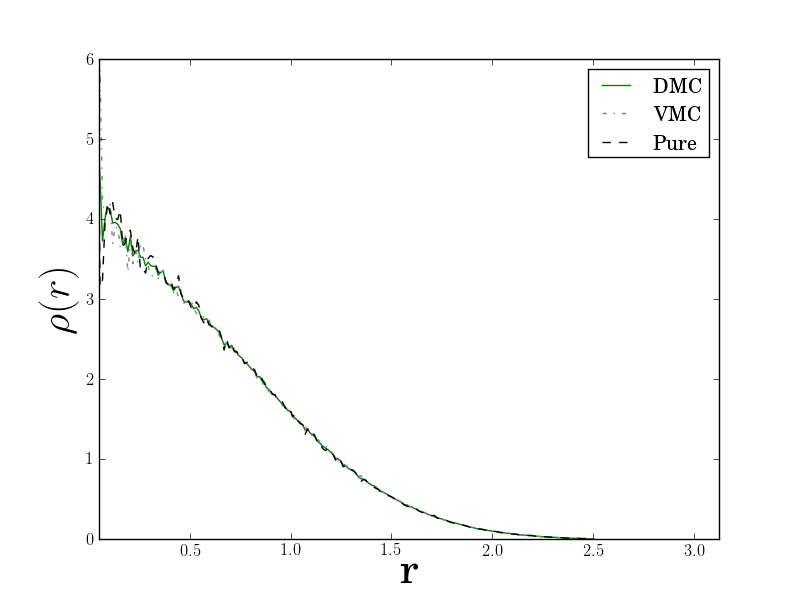
\includegraphics[scale=0.12]{../graphics/OBD/OBD_Q3D/QD2w1_2D.png}} &
   \subfigure{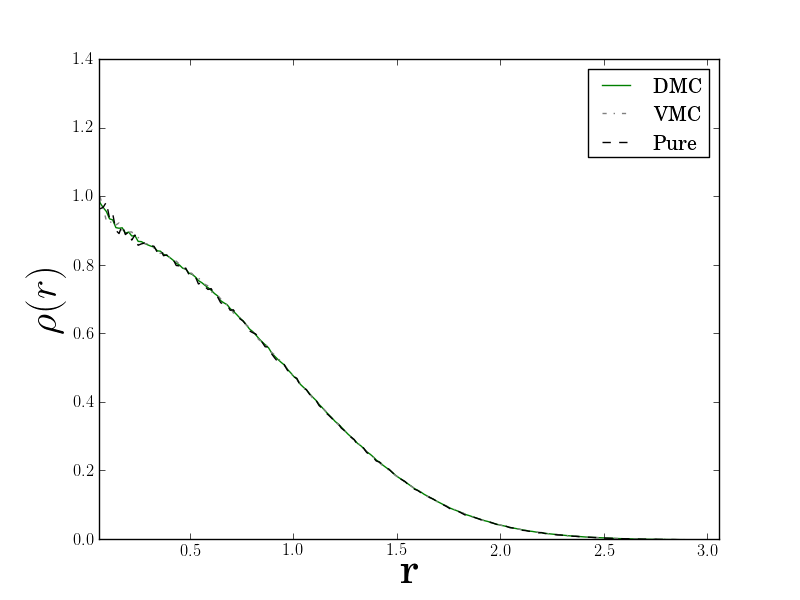
\includegraphics[scale=0.12]{../graphics/OBD/OBD_Q3D/comp/Q2D_2.png}} \\
   \subfigure{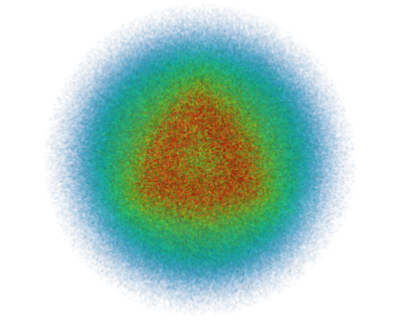
\includegraphics[scale=0.15]{../graphics/OBD/OBD_Q3D/QD8w1_3D.png}} &
   \subfigure{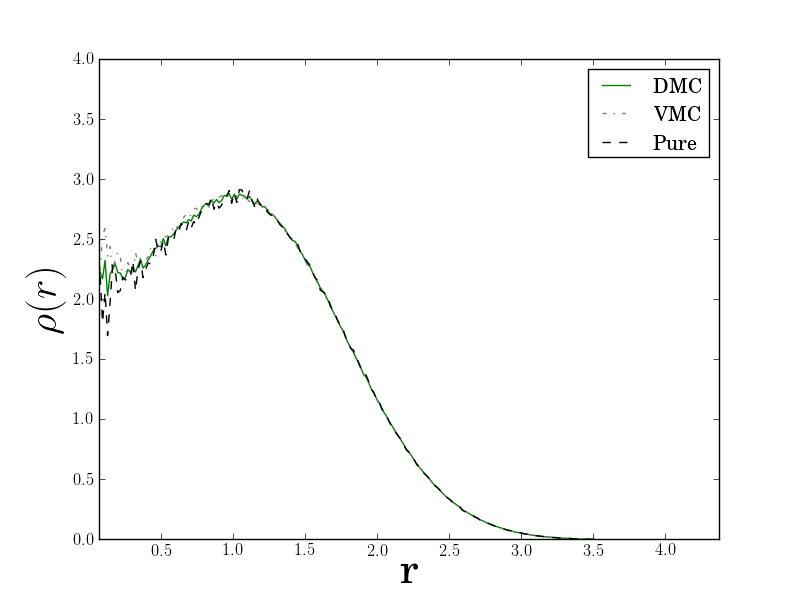
\includegraphics[scale=0.12]{../graphics/OBD/OBD_Q3D/QD8w1_2D.png}} & 
   \subfigure{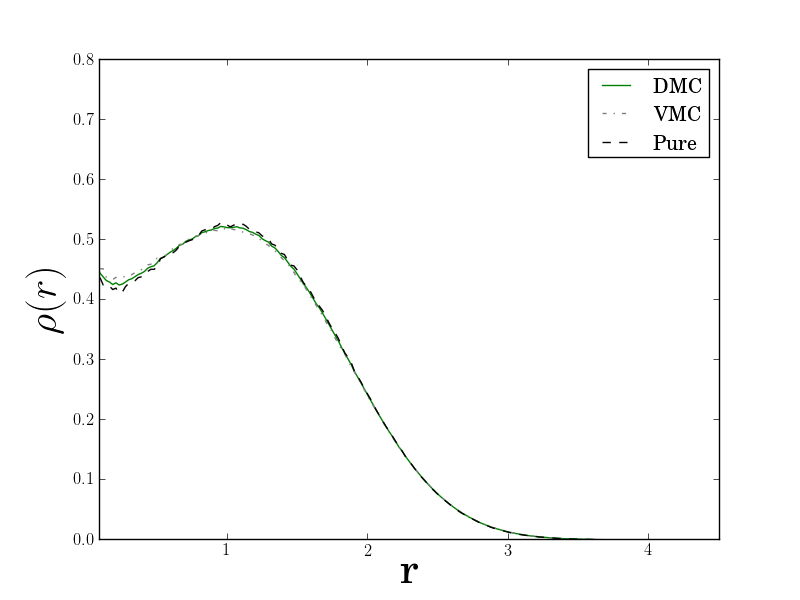
\includegraphics[scale=0.12]{../graphics/OBD/OBD_Q3D/comp/Q2D_6.png}} \\
   \subfigure{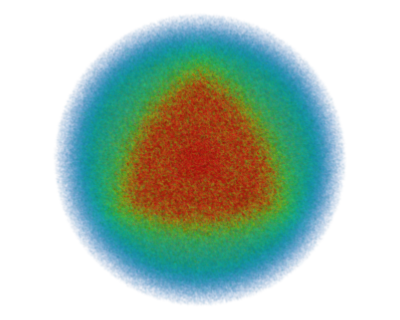
\includegraphics[scale=0.15]{../graphics/OBD/OBD_Q3D/QD20w1_3D.png}} &
   \subfigure{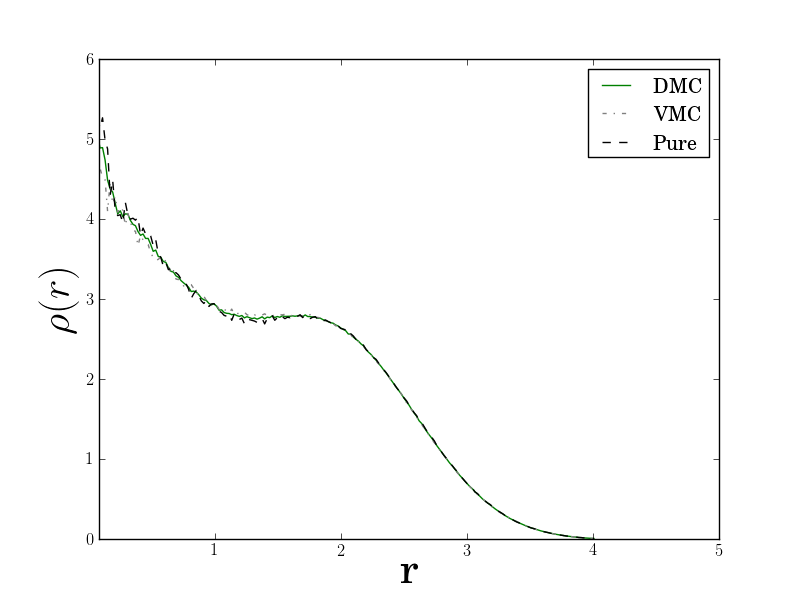
\includegraphics[scale=0.12]{../graphics/OBD/OBD_Q3D/QD20w1_2D.png}} & 
   \subfigure{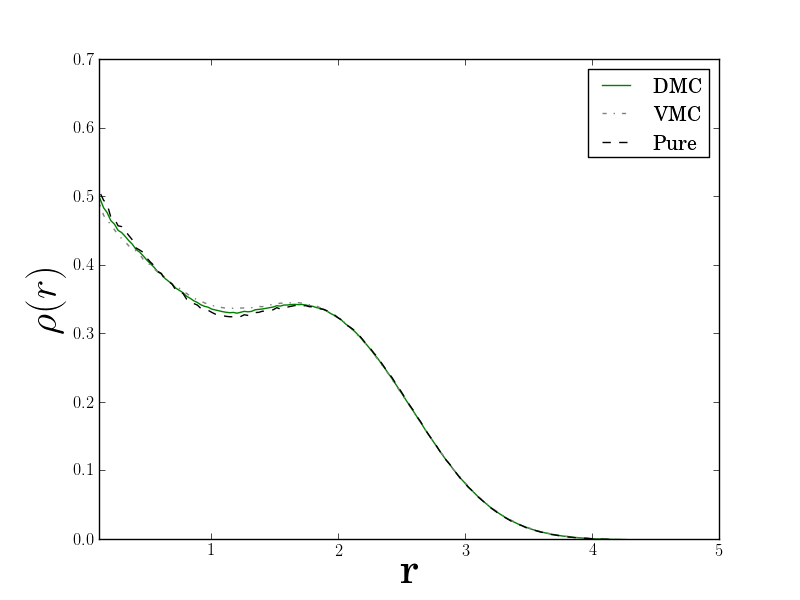
\includegraphics[scale=0.12]{../graphics/OBD/OBD_Q3D/comp/Q2D_12.png}} \\
  \end{tabular}
  \caption{One-body densities for two- and three-dimensional quantum dots.}
  \label{fig:OBD_QDOTS3D_highfreq}
 \end{center}
\end{figure}

\end{frame}


\begin{frame}
\frametitle{Lowering the frequency}

\setlength{\tabcolsep}{0.1pt}
\def\arraystretch{0}
\begin{figure}
 \begin{center}
 \begin{tabular}{rl}
   \footnotesize{\rot{$\qquad\omega=1$}}&\subfigure{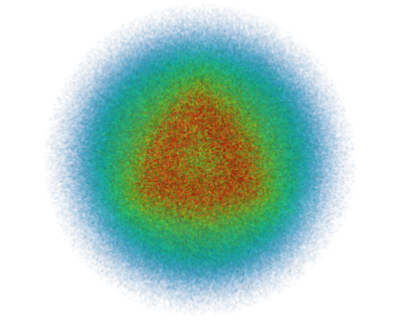
\includegraphics[scale=0.2]{../graphics/OBD/OBD_Q3D/QD8w1_3D.png}}
   \subfigure{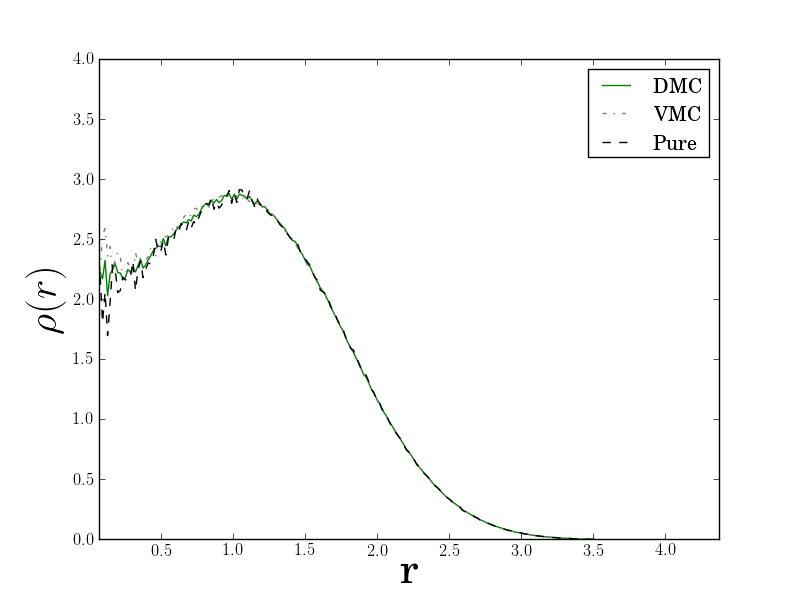
\includegraphics[scale=0.17]{../graphics/OBD/OBD_Q3D/QD8w1_2D.png}} \\
   \footnotesize{\rot{$\quad\,\,\omega=0.01$}}&\subfigure{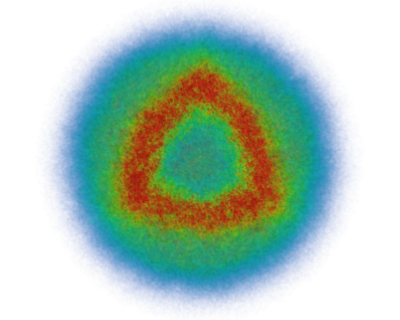
\includegraphics[scale=0.2]{../graphics/OBD/OBD_Q3D/QD8w001_3D.png}} 
   \subfigure{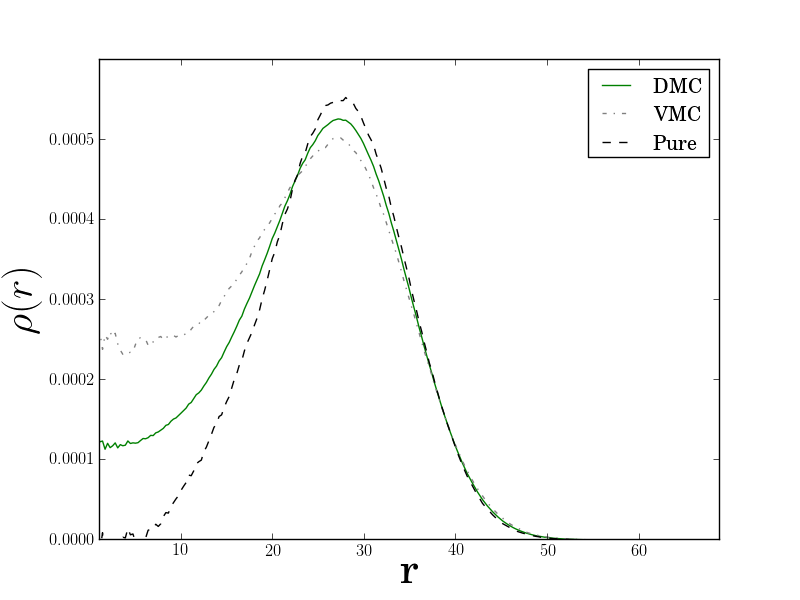
\includegraphics[scale=0.17]{../graphics/OBD/OBD_Q3D/QD8w001_2D.png}} 
  \end{tabular}
  \caption{One-body densities for a 8-particle three-dimensional quantum dot for high and low frequencies.}
  \label{fig:OBD_QDOTS3D_lowfreq}
 \end{center}
\end{figure}
\def\arraystretch{1}
\end{frame}


\begin{frame}

\captionsetup[subfloat]{labelformat=empty}

\tiny
\begin{figure}
 \begin{center}
 \begin{tabular}{rl}
  \rot{$\qquad\omega=0.28$}&\subfigure{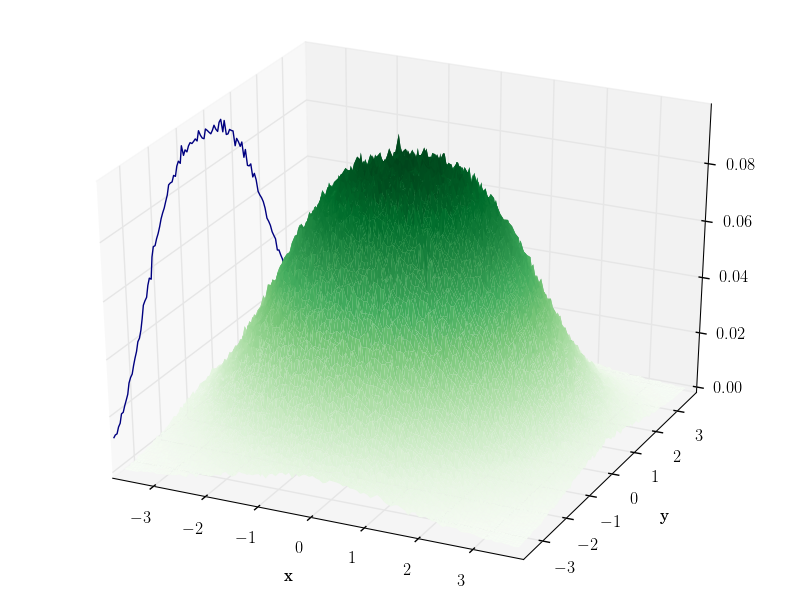
\includegraphics[scale=\OBDscale]{../graphics/OBD/OBD_DMC/dist_out_QDots2c028_3D.png}}
  \subfigure{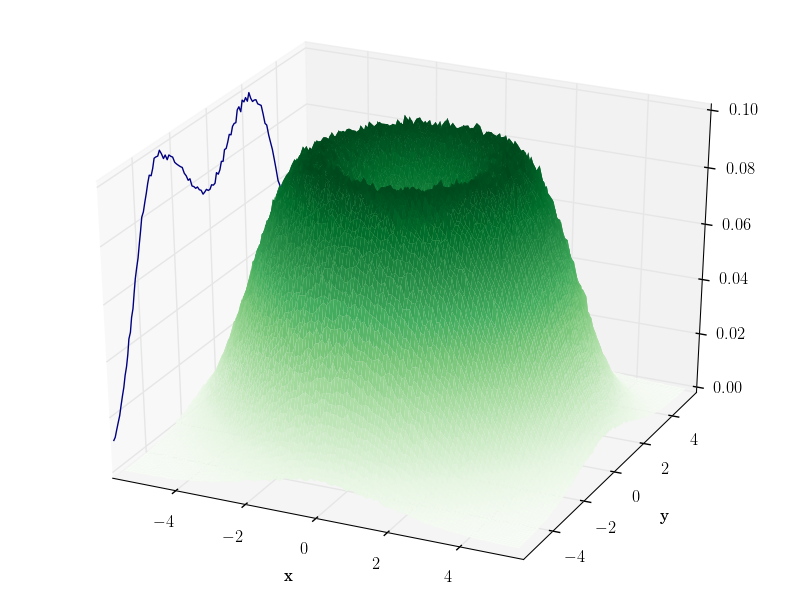
\includegraphics[scale=\OBDscale]{../graphics/OBD/OBD_DMC/dist_out_QDots6c028_3D.png}} 
  \subfigure{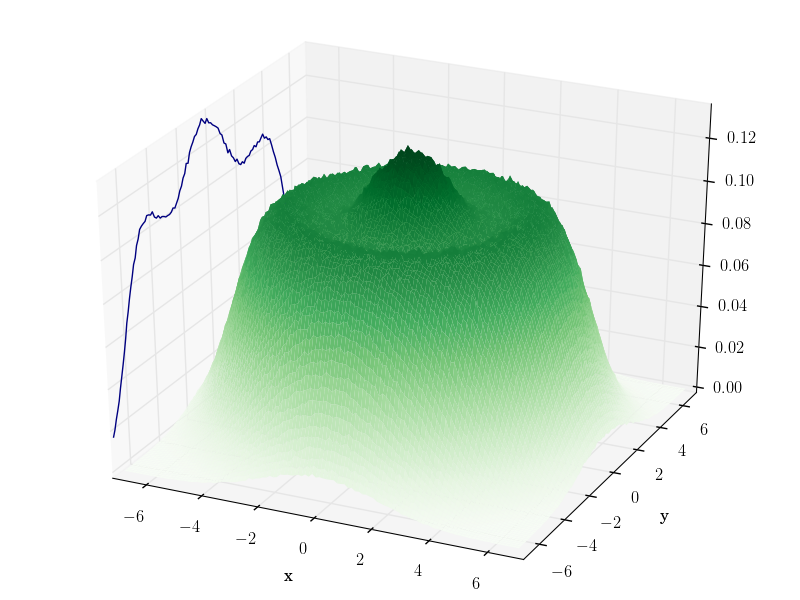
\includegraphics[scale=\OBDscale]{../graphics/OBD/OBD_DMC/dist_out_QDots12c028_3D.png}}
  \subfigure{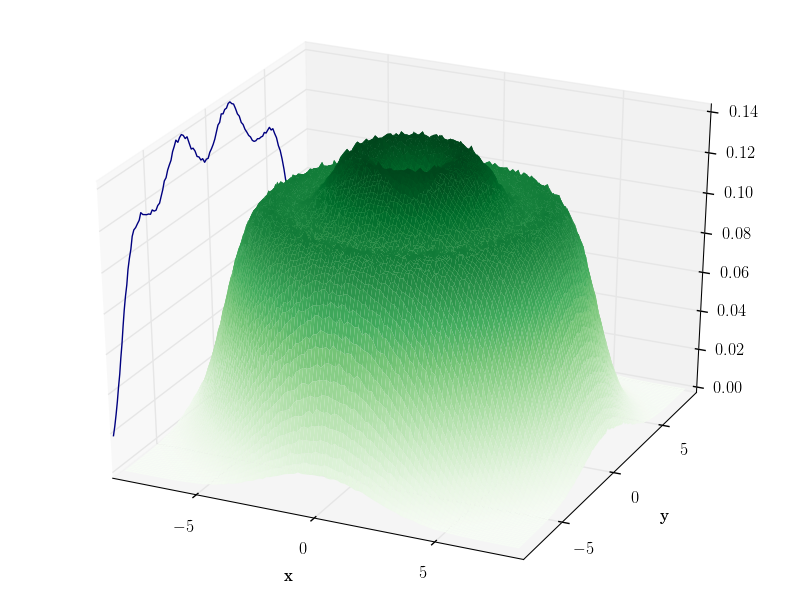
\includegraphics[scale=\OBDscale]{../graphics/OBD/OBD_DMC/dist_out_QDots20c028_3D.png}} \\[-0pt]
  \rot{$\qquad\omega=0.1$}&\subfigure{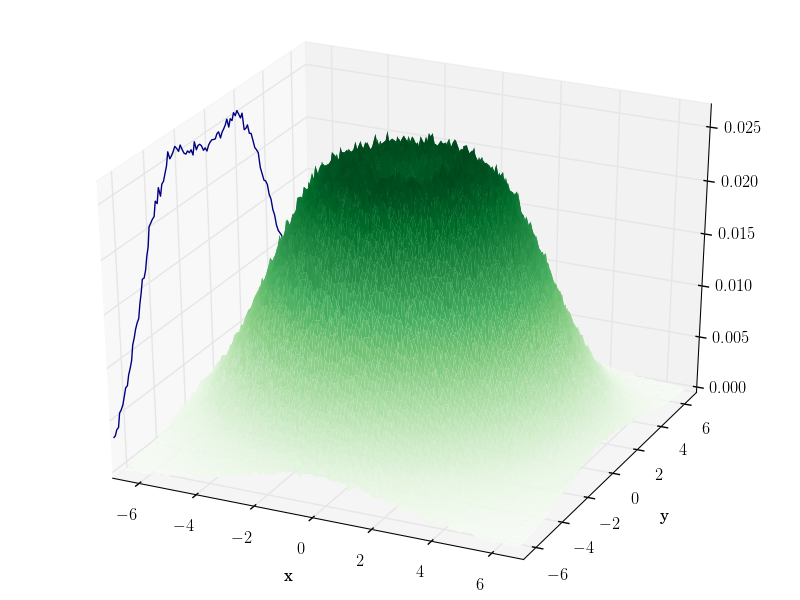
\includegraphics[scale=\OBDscale]{../graphics/OBD/OBD_DMC/dist_out_QDots2c01_3D.png}}
  \subfigure{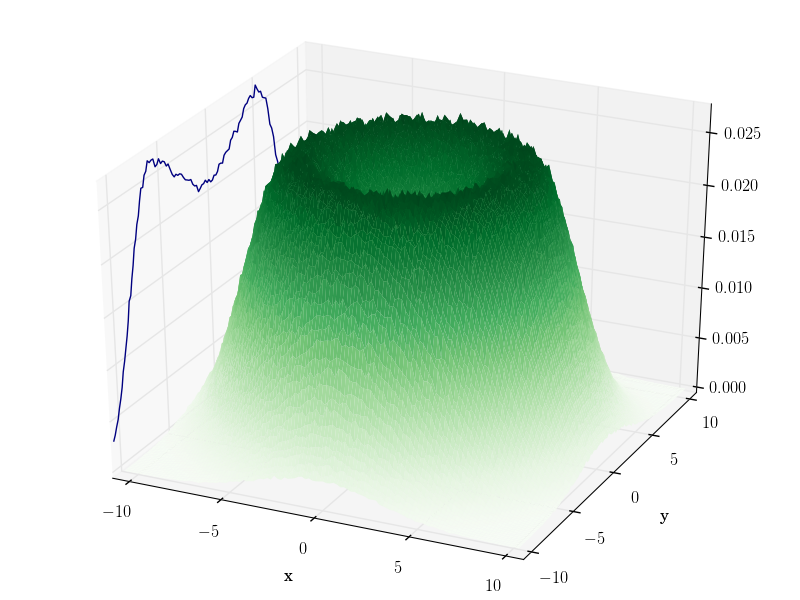
\includegraphics[scale=\OBDscale]{../graphics/OBD/OBD_DMC/dist_out_QDots6c01_3D.png}} 
  \subfigure{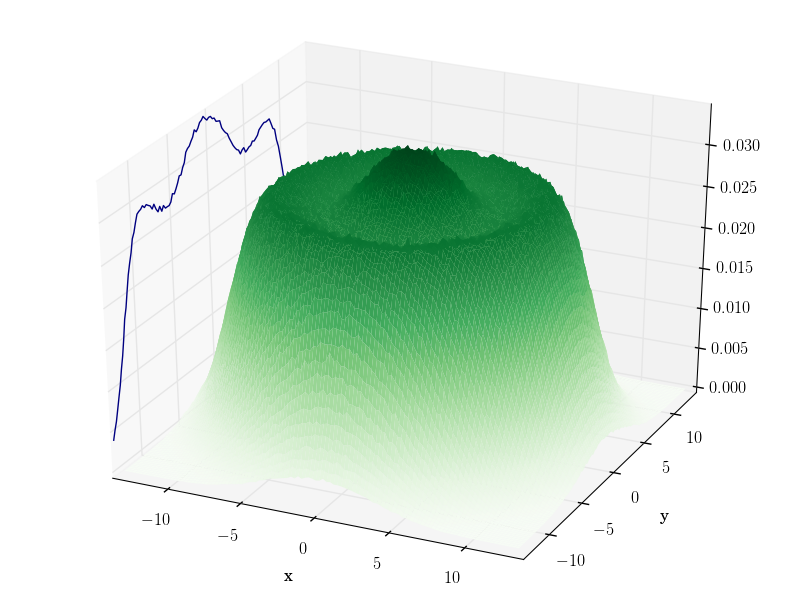
\includegraphics[scale=\OBDscale]{../graphics/OBD/OBD_DMC/dist_out_QDots12c01_3D.png}}
  \subfigure{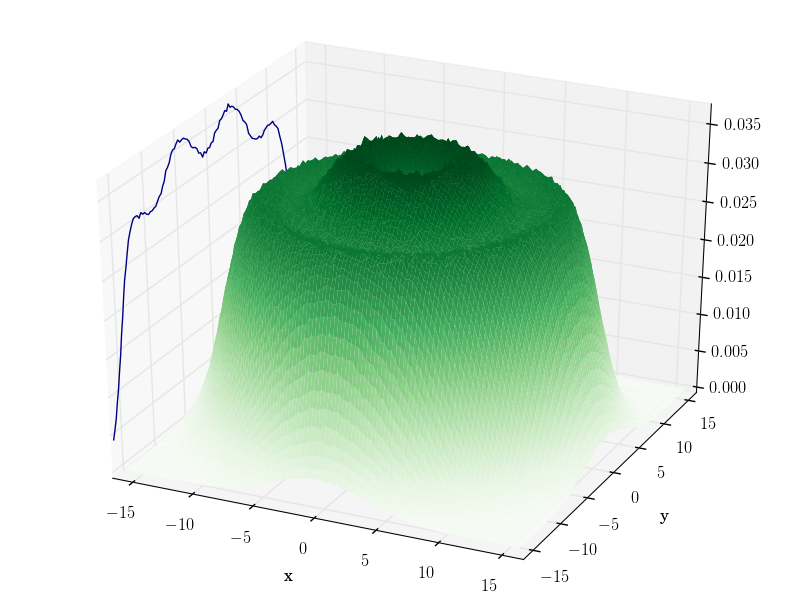
\includegraphics[scale=\OBDscale]{../graphics/OBD/OBD_DMC/dist_out_QDots20c01_3D.png}} \\[-0pt]
  \rot{$\qquad\omega=0.01$}&\subfigure[$N=2$]{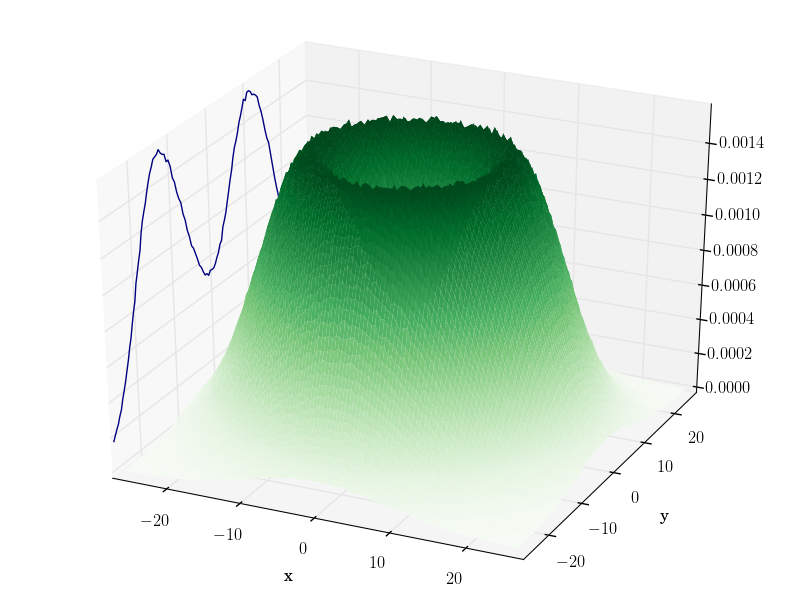
\includegraphics[scale=\OBDscale]{../graphics/OBD/OBD_DMC/dist_out_QDots2c001_3D.png}}
  \subfigure[$N=6$]{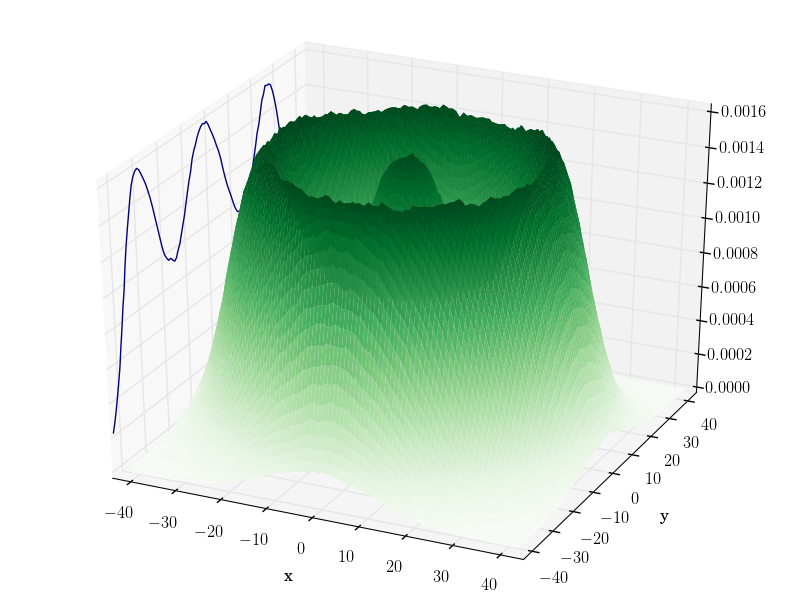
\includegraphics[scale=\OBDscale]{../graphics/OBD/OBD_DMC/dist_out_QDots6c001_3D.png}} 
  \subfigure[$N=12$]{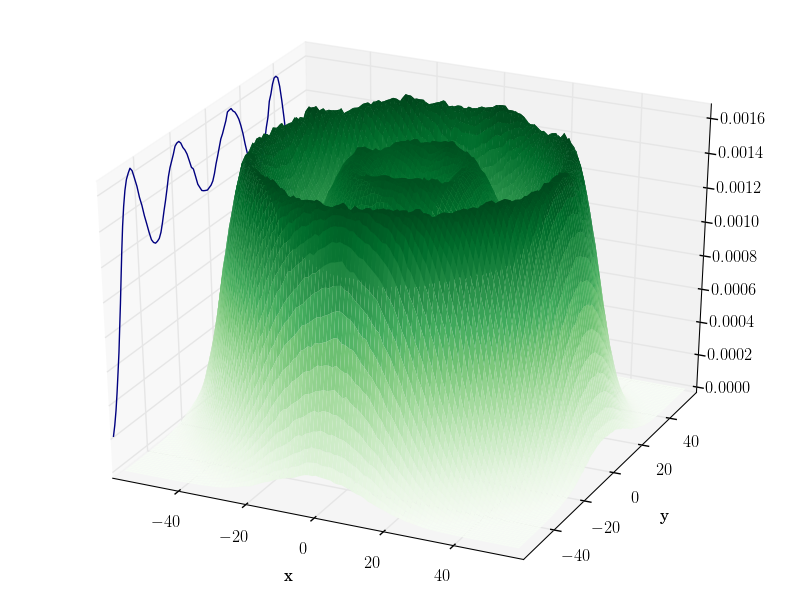
\includegraphics[scale=\OBDscale]{../graphics/OBD/OBD_DMC/dist_out_QDots12c001_3D.png}}
  \subfigure[$N=20$]{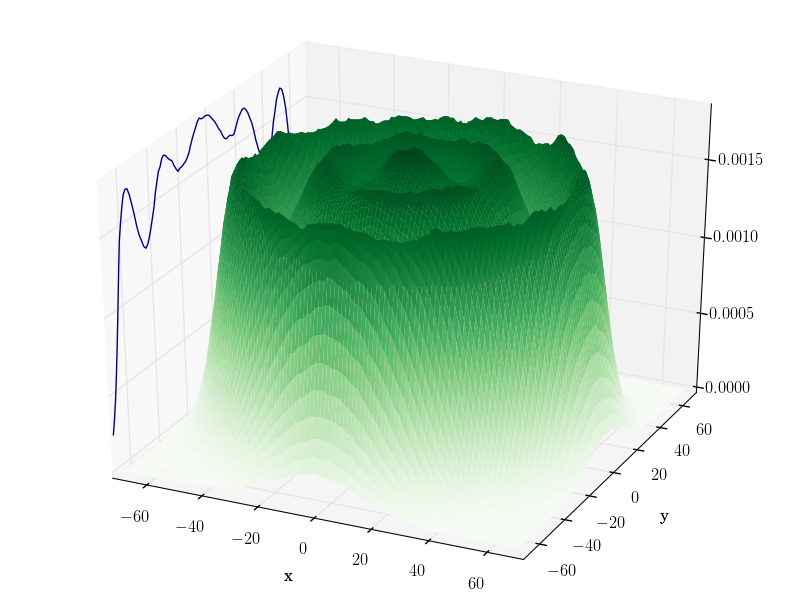
\includegraphics[scale=\OBDscale]{../graphics/OBD/OBD_DMC/dist_out_QDots20c001_3D.png}} \\
 \end{tabular}
  \label{fig:OBD_DMC_QDOTS_lowering3D}
 \end{center}
\end{figure}
\setlength{\tabcolsep}{6pt}
\normalsize

\end{frame}

\begin{frame}
 \begin{figure}
 \begin{center}
  \subfigure{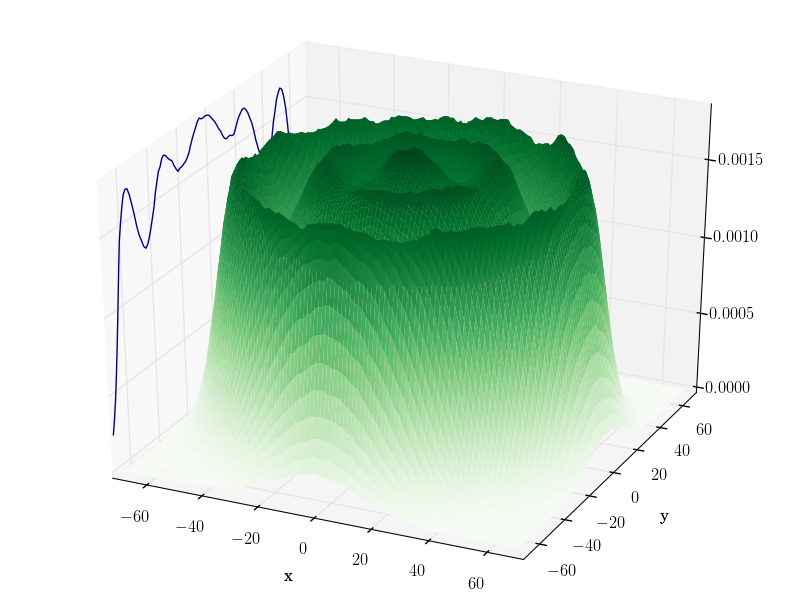
\includegraphics[scale=0.25]{../graphics/OBD/OBD_DMC/dist_out_QDots20c001_3D.png}}
  \subfigure{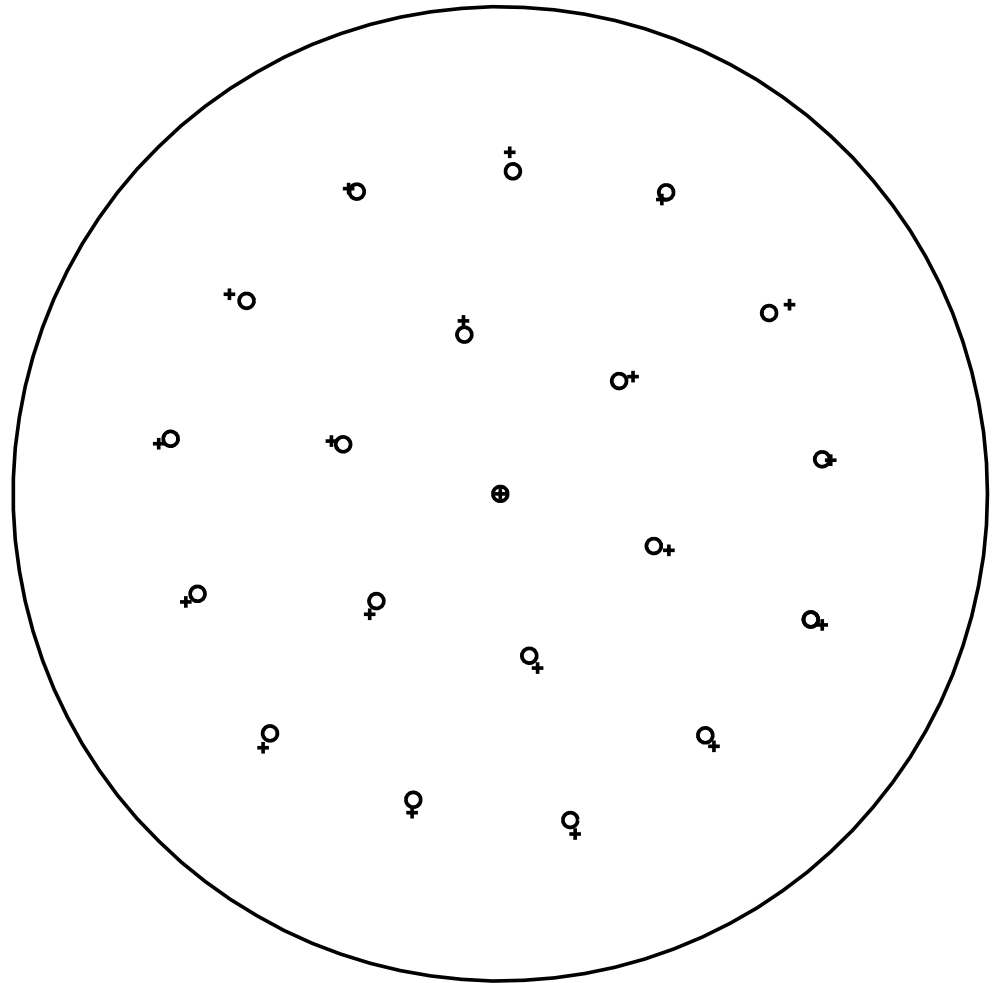
\includegraphics[scale=0.15]{../graphics/wigner/wigner20.png}}
  \label{fig:wigner20}
  \caption{OBD for a 20-particle two-dimensional quantum dot compared to the classical theoretical configuration taken from P. Galatola et al.~Eur. Phys. J. B \textbf{50}, 549 (2006)}
 \end{center}
\end{figure}
\end{frame}


\subsection{Atomic systems}

\begin{frame}
 asdasd
\end{frame}













